\documentclass{article}
\usepackage[utf8]{inputenc}
\usepackage{listings}
\usepackage{amsmath}

\title{An empirical study of semantic similarity in WordNet and Word2Vec}
\author{Abe Handler}
\date{\today}
\usepackage{graphicx}
\begin{document}

\begin{abstract}
Google's unsupervised Word2Vec system attempts to determine the semantic distance between words at web scale. This paper performs an empirical analysis of Word2Vec's determinations by comparing them to WordNet, a well-known, human-curated lexical database. It finds that Word2Vec tends to uncover more of certain types of semantic relations than others, with Word2Vec returning more hypernyms than synonyms followed by meronyms, hyponyms and holonyms. Moreover, it shows the likelihood that neighbors separated by distance k in Word2Vec are semantically related in WordNet.
\end{abstract}

\maketitle

\section{Introduction}

\[
0.0626\times\ln{(x)} + 0.0097
\]

Computer scientists have spent decades attempting to discern semantic relationships between different words\footnote{techniques include latent semantic indexing and Latent Dirichlet allocation}. One new unsupervised system, Word2Vec, has attracted lots of recent attention\footnote{garnering over 100 citations in the year since its publication in 2013}. However, certain aspects of its output are poorly understood. In particular: 

\begin{enumerate}
\item Word2Vec does not label particular semantic relationships between words -- like the synonomy between \textit{cold} and \textit{chilly} or the meronomy between \textit{wheel} and \textit{car}. Instead, it assigns a number between 0 and 1, indicating the semantic distance\footnote{For instance, a Word2Vec model trained on the Google news corpus returns a semantic distance of .390 between \textit{truck} and \textit{tire} and a semantic distance of .168 between \textit{truck} and \textit{chicken}} between two words. However, as Word2Vec’s creators note ``there can be many different types of similarities.” \cite{mikolov2013efficient} This opens a question: what sorts of semantic similarities does Word2Vec uncover?
\item What is the relationship between the semantic distance of two words in Word2Vec and the likelihood that those words stand in some semantic relationship? For instance, how much more likely are you to find a synonym on the k-th closest neighbor, as opposed to the k * 2 -th neighbor?
\end{enumerate}

This study seeks to answer such questions by comparing Word2Vec's output with WordNet -- a large, human-curated ``lexical database" \cite{Wordnetwebsite} and the most-frequently cited ``lexiographic resource" \cite{widdows} in English. Unlike Word2Vec, which represents words as vectors, WordNet models language with a large graph -- with semantically similar words (caled ``synsets") serving as the nodes and semantic relationships (such as the meronomy between \textit{tire} and \textit{car}) serving as the edges. 

Understanding the relationship between semantic similarity in WordNet and Word2Vec has two motivations. First, the study simply gives clearer knowledge of Word2Vec, which is still not well understood. Second, the study shows how Word2Vec may be used to make more optimal use of WordNet. Because WordNet look ups are expensive, applications could use a (quickly-calculated) semantic distance in Word2Vec as a quick test to determine the likelihood of am match before searching WordNet. Finally, as researchers and pracitioners build semantic tools from Word2Vec they will inevitably turn to WordNet to benchmark and evalaute their applications. Understanding Word2Vec's output will make their evaluations much more accurate. 

\section{Related Work}

\subsection{Word2Vec}
Word2Vec uses complex, multi-level neural networks to determine semantic distance. It's output is a  space filled with vector representations of words. Word vectors that are closer together are more closely related than word vectors that are farther apart. 

The approach has garnered lots of attention and enthusiasm. Over 100 researchers have cited Word2Vec since 2013. Researchers have tried using Word2Vec to find the dominant sense of a word (determine the meaning of a word in context) \cite{wang2014introduction}. They have tried to use Word2Vec to perform sentiment analysis (automatically determine attitudes) \cite{xue2014study}. Some have even tried to use Word2Vec to ascertain political ideology \cite{iyyerpolitical}. However, no empirical studies have yet attempted to systematically analyze output from Word2Vec in terms of the classical tool, WordNet. 

The reason this is necessary is that that WordNet remains the best automated method for determining precise semantic relationships. As researchers build exciting new tools from Word2Vec they will almost certainly turn to WordNet to check the output from their applications. For instance, Rei et. all \cite{rei2014looking} use Word2Vec as part of a hyponym detector in their ``Looking for Hyponyms in Vector Space" -- look to WordNet to evaluate their method. However, their evaluation presupposes certain relationships between WordNet and Word2Vec without providing any empirical justification. The authors assume that ``the most likely candidates for a high cosine similarity are synonyms, antonyms, hypernyms and homonyms". However, in section \ref{binary} we show that Word2Vec does not in fact return these semantic relations with equal likelihood. A clearer understanding of how WordNet and Word2Vec are related will yield much cleaner and more precise evaluation of tools built on top of Word2Vec. After all, both the linguistic mechanisms and the exact output of the Word2Vec system are still a bit mysterious. One popular explanation of the system concludes: ``Why does this produce good word representations? Good question. We don’t really know." \cite{goldberg2014word2vec}

\subsection{WordNet}  \label{WordNet}
WordNet has been a part of natural language processing for decades -- beginning at Princeton University in 1986. The system has its own logic and jargon, all built around the fundamental building block \cite{wordnet} of the ``synonymous set" (or synset) -- an unordered collection of ``cognitively synonymous words and phrases." \cite{cruse} Synsets are linked by relations, with particular relations linking particular words with particular parts of speech. \footnote{Because ``the majority of the WordNet’s relations connect words from the same part of speech (POS) ... WordNet really consists of four sub-nets, one each for nouns, verbs, adjectives and adverbs, with few cross-POS pointers."\cite{Wordnetwebsite}}

Five specific WordNet relationships concern us here:

\begin{itemize}

  \item \textbf{Synonomy}. WordNet can identify synonyms, words with the same meaning. For instance: \textit{roof} and \textit{ceiling}.
  \item \textbf{Hypernomy}. A word that is more general than some other word is said to be its hypernym. \textit{Language} is a hypernym of \textit{French}
  \item \textbf{Hyponomy}. A word that is more specific than some other word is said to be its hyponym. \textit{French} is a hyponym of \textit{language}
  \item \textbf{Meronomy}. A word that is a part of some other word is called a meronym. \textit{Bedroom} is a meronym of \textit{house}.
  \item \textbf{Holonomy}. If B contains A, B is a holonym of A. \textit{Japan} is a holonym of \textit{Fuji} because Fuji is in Japan.
\end{itemize}

Note that these are relationships between synsets, not between words. A word is associated with one or more synsets. A synset has a semantic relationship with other synsets. We explain our exact definition of semantic relation in the section \ref{method}

\section{Method} \label{method}
If word vectors represent semantic similarity, we might expect a that word's k-nearest neighbors in Word2Vec have some semantic relationship in WordNet. Moreover, the exact nature of these semantic relationships is unknown. We investigate each of these hypotheses with the following experiment. 

We begin with Google's word model, trained on 100 billion words in the Google news corpus \cite{Word2VecWebsite}. Then we randomly select 10,000 words from the Reuters news corpus and, for each, we search for the closet 1000 neighbors in the Word2Vec model. We then search WordNet for any semantic relationship between the original word and its neighbor. We only concern our self with the semantic relations listed in section \ref{WordNet}. 

We allow two words to stand in multiple semantic relationships. For instance, a word is permitted to be both a hyponym and a holonym, if so labeled in WordNet. We also keep track of words that do not appear in WordNet and words that have the same stem -- like \textit{nearing} and \textit{nears}. In these two cases, we do not search for the semantic relationships in WordNet because the relationship is already known. We do not consider antonyms as Wordnet defines anyonyms between words -- not between synsets -- and all other relations are defined between synsets. 

We access WordNet and the Reuters corpus with the Python linguistics toolkit, NLTK \cite{BirdKleinLoper09}. We access the Google news model via the popular python wrapper, Gensim \cite{gensim}. We use NLTK's snowball stemming tool to find words with the same stem. 

We use a binary measure to determine semantic relatedness in WordNet: if there is any overlap between the relevant synsets, we count the relation. If there is zero overlap between the synsets, we do not count the relation. For instance, our experiment might determine that \textit{introduction} and \textit{initiation} are synonyms because their synsets overlap with the synset 'initiation.n.01' -- defined as 'a formal entry into an organization or position or office'. 

This opens a potential complicating problem: the simple binary determination does not take into account that the word ``introduction" has seven associated synsets, but the word ``initiation" has only 4 synsets -- and that these two sets overlap on a single synset. To account for the relative degree of overlap, we also take the Jaccard index of the overlapping sets to gain a better sense of the degree to which semantically related words are related.

Finally, we again randomly sample 10,000 words from the Reuters corpus and determine the average number of synonyms, meronyms, holoynms, hypernyms and hyponyms in WordNet. We show the relative sizes of each type of relation in WordNet and use these to adjust the count of relations from Word2Vec. For instance, a word has, on average, 11 times fewer holonyms than hyponyms in WordNet. We use these ratios to generate \textbf{adjusted counts} of each word that show how many of each relation Word2Vec would find if each type of relation was equally present in WordNet.

We also uses there relative sizes to examine the Jaccard indexes, demonstrating that such indixes indicate more about the structure of WordNet than about the nature of relationships from Word2Vec.

\section{Results}

\subsection{What kinds of relations does Word2Vec uncover?} \label{binary}
In general, Word2Vec finds more synonyms, hyponyms and hypernyms than meronyms and holonyms (counting any overlap in appropriate synsets as a relation). The overall pattern is shown in Fig. \ref{fig:all} on page \pageref{fig:all}.
\begin{center}
\centering
    \begin{tabular}{ | l | l | l | l | l | l |}
    \hline
Relation & k less than 200 & k=200-400 & k=400-600 & k=600-800 & k=800-1000 \\  \hline
Holonomy &351 & 118 & 78 & 53 & 48\\  \hline
Meronomy &572 & 152 & 97 & 88 & 72\\  \hline
Hyponomy &6454 & 2093 & 1453 & 1118 & 949\\  \hline
Synonomy &8980 & 2266 & 1448 & 1092 & 939\\  \hline
Hypernomy &10644 & 3765 & 2461 & 2024 & 1737\\  \hline
Same stem &17312 & 1903 & 1149 & 816 & 630\\  \hline
    \end{tabular}
\end{center}
\begin{figure}[!hb]
  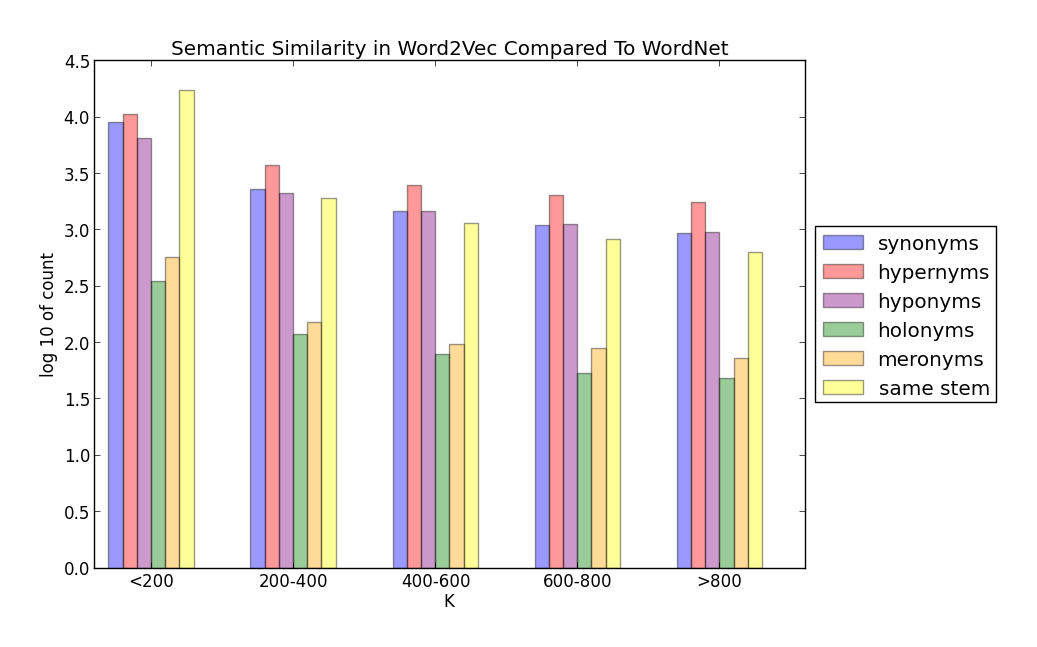
\includegraphics[scale=.5]{all.png}
  \caption{Word2Vec finds more hypernyms and synonyms than meronyms, hyponyms and holonyms. It finds fewer of all of the kinds of relations as k increases, meaning that words are less likely to be related in WordNet as their semantic distances grow farther away.}
  \label{fig:all}
\end{figure}
Two forms of relation deserve particular note. 


\begin{enumerate}
  \item We find that by far the largest category are those results that do not appear at all in WordNet. This is because the model trained on the Google news corpus with Word2Vec is much, much larger than all of WordNet. Where WordNet 2.1 contains around 118,000 synsets \cite{wordnet}. The Word2Vec model in this experiments was trained on 100 billion words \cite{Word2VecWebsite} of news text. Most of the semantically similar words cannot be looked up in WordNet. For instance, \textit{Rohto Pharmaceutical} is not in WordNet: it's a big corporation, but not a household name in the United States. Thus WordNet has no way of determining its semantic relationship to the word \textit{industries}.\footnote{The Google news Word2Vec model lists the semantic distance between \textit{Rohto Pharmaceutical} and \textit{industries} at .494} It is not known how well the WordNet relations represent the mass of `semantically similar' words in Word2Vec. We consider this in section \ref{Future Work}.
\item Word2Vec finds many words with the same stem when k is small. But as k decreases, the number of words with the same stem decrease quickly, as shown in figure \ref{fig:same_stem}.
\end{enumerate}

\begin{figure}[!hb]
\centerline{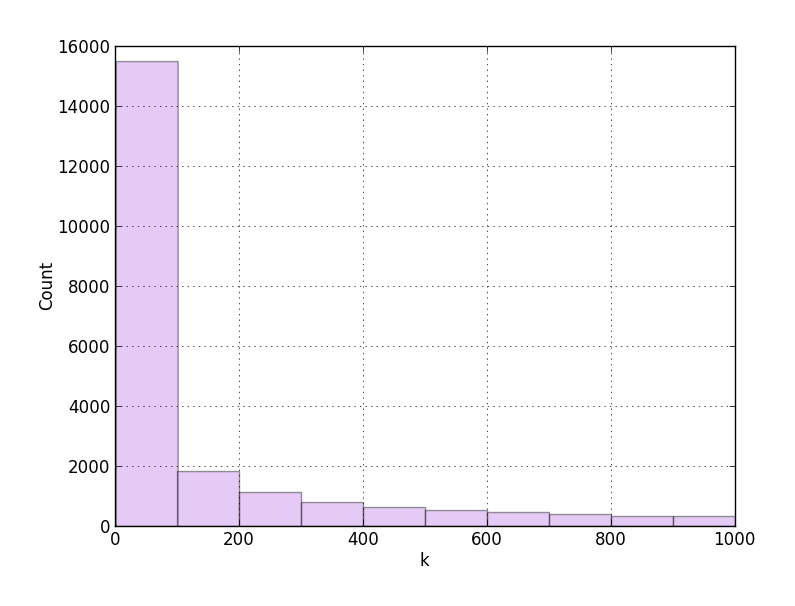
\includegraphics[scale=.5]{Same_stem.png}}
  \caption{Word2Vec finds many words with the same stem at small values of k. But this number falls off quickly as k increaes.}
  \label{fig:same_stem}
\end{figure}


\subsection{Values of K} \label{val_k}
There are far fewer WordNet relations across all categories as k gets larger.  In other words, the greater the semantic distance (in Word2Vec), the greater the value of k and the less likely that two words are semantically related in WordNet. This is as expected, provided that Word2Vec's determinations of semantic distance are reliable.

\begin{figure}    
\begin{minipage}[t]{0.45\textwidth}
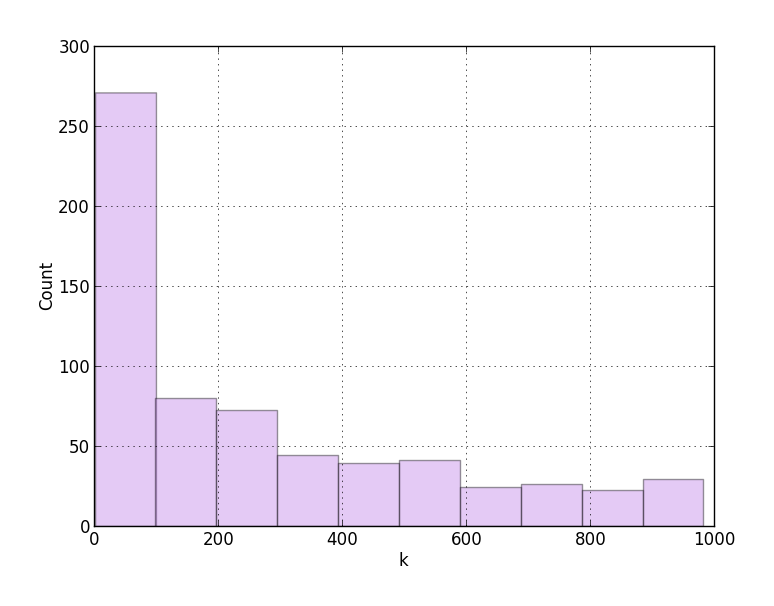
\includegraphics[width=\linewidth]{Holonym_Distance.png}
\caption{Count holonyms by k}
\label{fig:holonyms}
\end{minipage}
\hspace{\fill}
\begin{minipage}[t]{0.45\textwidth}
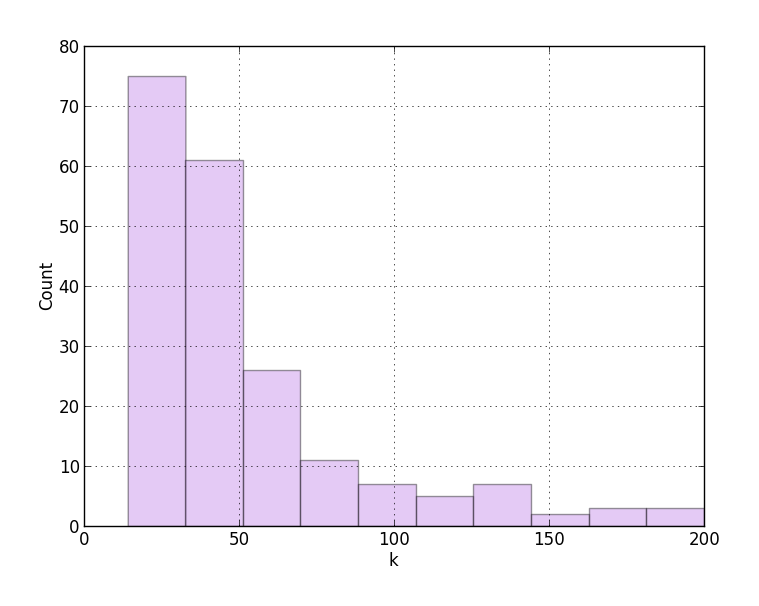
\includegraphics[width=\linewidth]{Hypernym_Distance.png}
\caption{Count hypernyms by k}
\label{fig:hypernyms}
\end{minipage}

\vspace*{0.5cm} % (or whatever vertical separation you prefer)
\begin{minipage}[t]{0.45\textwidth}
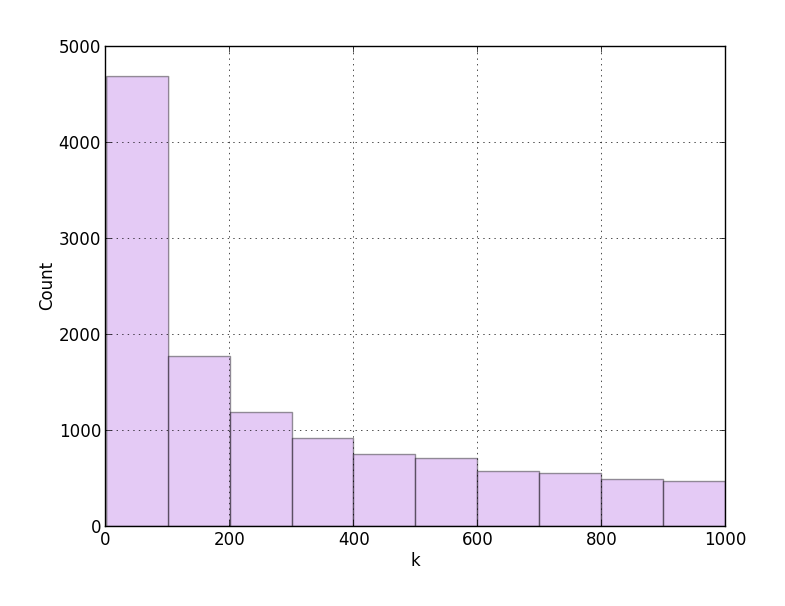
\includegraphics[width=\linewidth]{Hyponym_Distance.png}
\caption{Count hyponyms by k}
\label{fig:hyponyms}
\end{minipage}
\hspace{\fill}
\begin{minipage}[t]{0.45\textwidth}
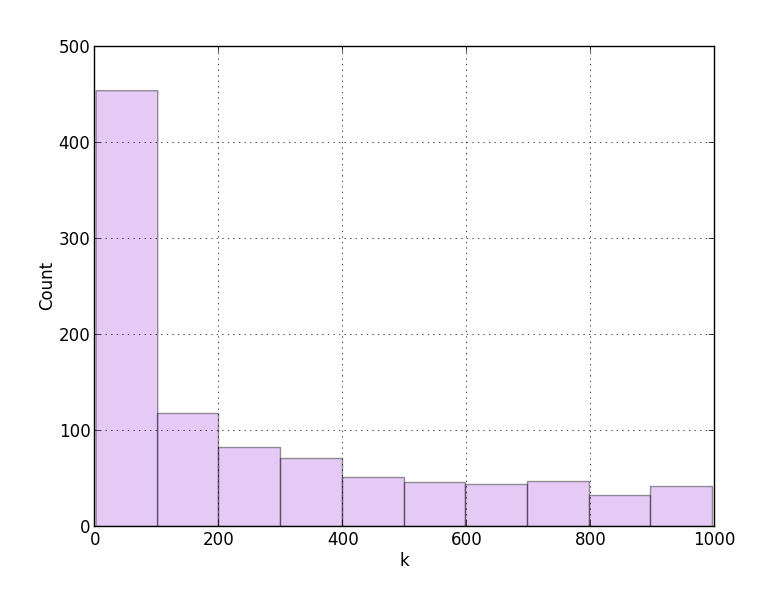
\includegraphics[width=\linewidth]{Meronym_Distance.png}
\caption{Count meronyms by k}
\label{fig:meronyms}
\end{minipage}
\caption{For all types of relations, the number of relations drops as k increases. As words are further apart in Word2Vec they are less likely to be related in WordNet}
\end{figure}

\subsection{Degree of overlap}
Results in section \ref{binary} consider any overlap between synsets as a  ``relation". For instance, consider a given word pair A,B. Imgine that Wordnet gives 3 synsets as hyponyms of A and gives 5 synsets for B. If one of the synsets that are hyponyms of A matches one of the 5 synsets for B then we consider this a hyponym. However, are certain types of relation closer than others? We investigate this by examining the Jaccard coefficient of each linked relation -- i.e. the intersection of two sets divided by their union. Our findings are shown in figure \ref{fig:jacard}.

\begin{figure}[!ht]
\centerline{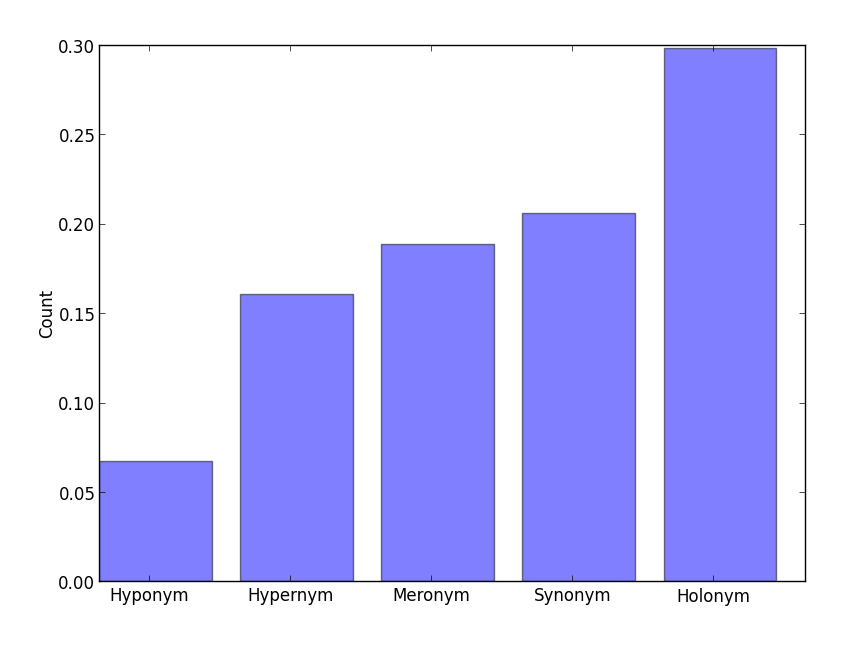
\includegraphics[scale=.5]{jacard.png}}
  \caption{Jaccard indexes vary depending on type of relation -- but the variation is closely correlated to the different sizes of synsets in WordNet}
  \label{fig:jacard}
\end{figure}

At first glance, figure \ref{fig:jacard} seems to show that Jacard indexes vary. However, we sampling 10,000 words from the Reuters corpus and finding the average number of synonyms, hypoynms, hypernyms, holonyms and meronyms associated with each word (excluding zeros) shows that Jaccard indexes for a given type of relation are strongly linked with the average synset sizes for each type of relation in WordNet.

\begin{center}
\centering
    \begin{tabular}{ | l | l |}
    \hline
Relation & Relative sizes of types of synsets in Wordnet \\  \hline
Synonomy & .141 \\  \hline
Hyponomy & .576  \\  \hline
Hypernomy & .132 \\  \hline
Holonomy & .049 \\  \hline
Meronomy & .100 \\  \hline
    \end{tabular}
\end{center}

In other words, the Jaccard index for holonyms is highest -- but the holonymm set has the lowest average size in WordNet. This means that for holonyms, the denominator in the index will be smaller and the overall value will be greater. Similarly, the Jaccard index for hyponyms is lower because the average number of hyponyms is greater. Differences in Jaccard indexes seem largely attributable to differences in synset sizes in WordNet (or perhaps in English), not to differences in the semantic relations uncovered by Word2Vec.

\subsection{Adjusted counts}
To what extent do differences in the relative synset sizes explain the different sorts of relations uncovered by Word2Vec? For instance, if words have more synonyms than holonyms, then it would make sense for Word2Vec to find more synonyms than holonyms. Thus, we revisit the results from section \ref{binary} with adjusted counts.

To find an adjusted count, we take the average number of each type of relation returned for a particular word. We find the max of each of those numbers. And, for each relation that is not the maximum, we find that number as a fraction of the maximum. The adjusted count is 1 over the inverse of that number times the actual count. So if the average synset size for meronyms is 1/4 smaller than the average synset size of hyponyms (the biggest), the meronym count would increase by 1/.25 = 4.

\begin{figure}[!ht]
  \begin{minipage}{0.7\textwidth}
    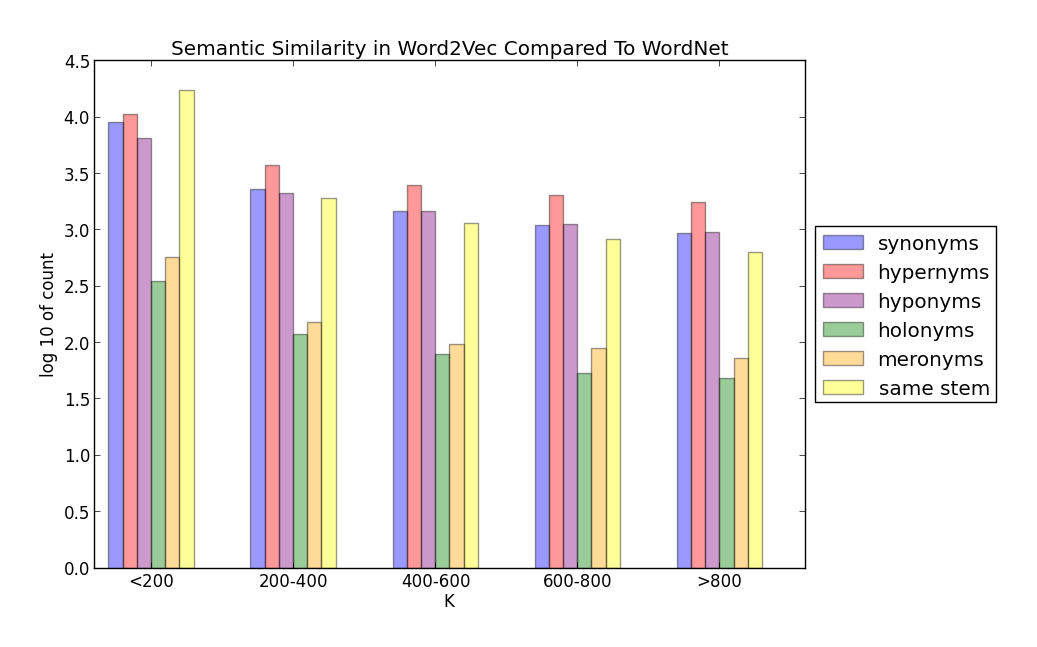
\includegraphics[width=\textwidth]{all.png}
    \caption{Counts from section \ref{binary}}
  \end{minipage}
 
  \begin{minipage}{0.7\textwidth}
    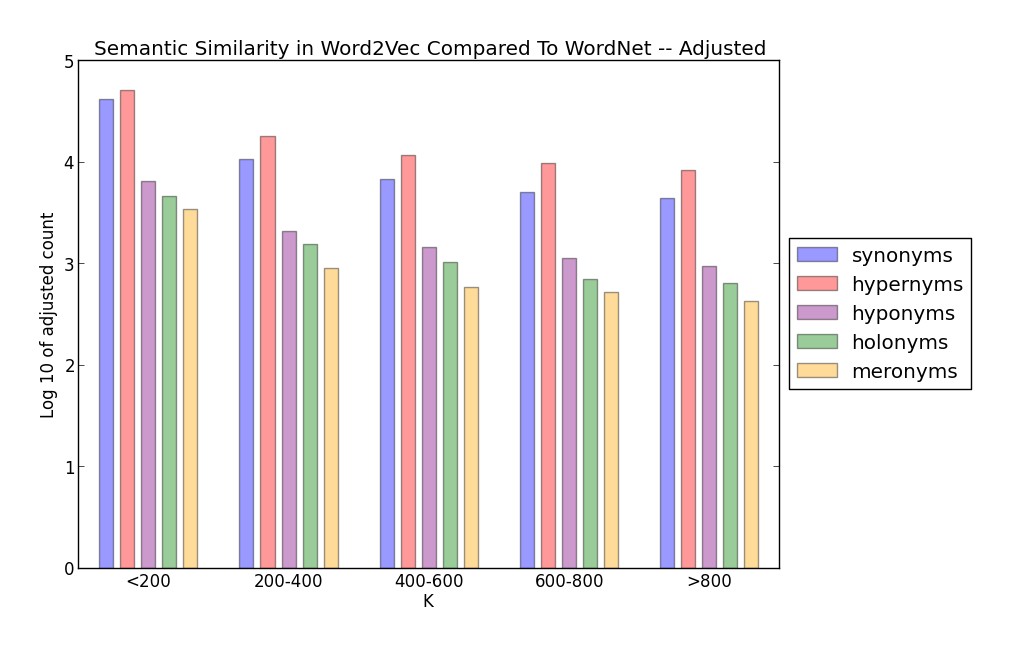
\includegraphics[width=\textwidth]{Adjusted.png}
    \caption{Counts adjusted for synset size}
  \end{minipage}
\end{figure}

Adjusted counts give a different perspective on Word2Vec. They show that, in general, Word2Vec returns more hypernyms than synonyms -- followed by hypernyms, holonyms and meronyms. 

\subsection{Likelyhoods}
It might be possible to consider the likelihood of a given relation at a particular value of k. We consider this in \ref{fig:likelyhood}

\begin{figure}[!ht]
\centerline{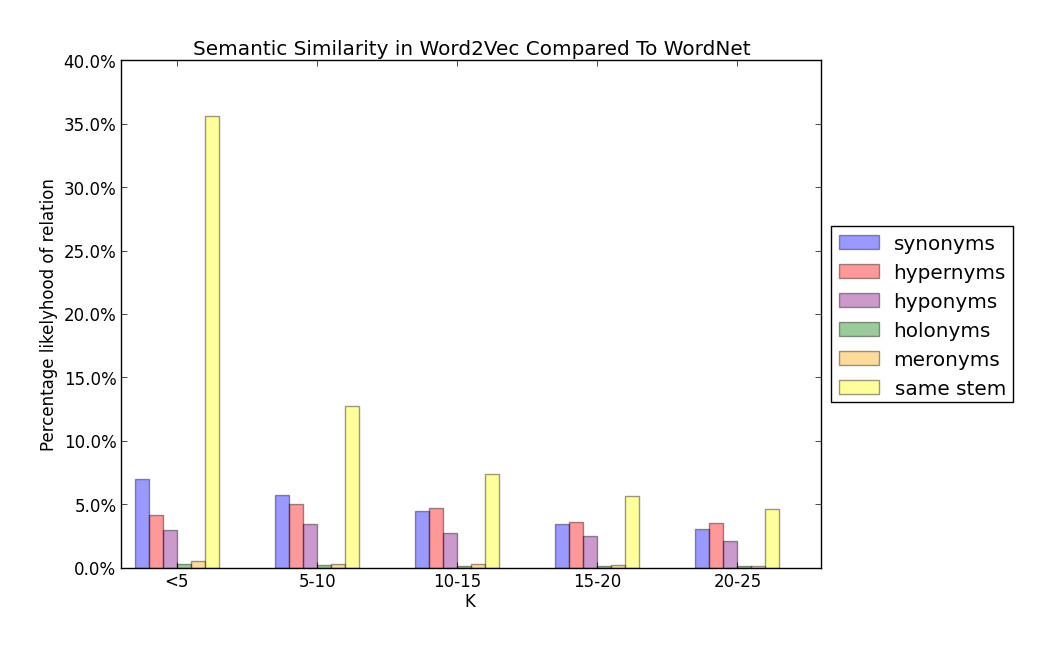
\includegraphics[scale=.5]{Likelyhood.png}}
  \caption{Different likelihoods at different values of k}
  \label{fig:likelyhood}
\end{figure}


\section{Future Work} \label{Future Work}

Unsupervised natural language processing is progressing quickly. Systems like \cite{PATTY} and \cite{ReVerb2011}

The semantic categories in WordNet have been a part of linguistics and philosophy since at least the time of Aristotle. Are the categories insufficiently granular? Does Word2Vec capture meaningful similarities that are not included in WordNet? Or is Word2Vec off? How would you measure this? 

-Synonym might be vague. Autumn, fall. Are these semantically closer than case and box? What about other senses of a word?  Box has many different connotations. Word2Vec find this? 

Sample the relations?

\bibliographystyle{unsrt}%Used BibTeX style is unsrt
\bibliography{sample}

\end{document}
